
\chapter{Related Work} \label{ch:related-work}

Relevant papers originate from two lines of work: On one hand additions to refinement types for mutability, asynchronous execution etc. and on the other verification frameworks for Rust.


% Of course the design space permits choosing other tradeoffs. For example, Rondon et al. \cite{rondon_low-level_2010} choose
%   - only interdependence in single record using fold mechanism
%   - 


\paragraph*{Refinement Types} Refinement Types were originally developed for verification in functional languages by Freeman and Pfenning \cite{freeman_refinement_1991}, who define a subtyping relation for ML types on a lattice of possible union and intersection of types and check them using a system called tree automata. 
Xi and Pfenning \cite{xi_dependent_1999} rephrase this notion subtype refinement as a restricted dependent type, where the constraints less expressive than the base language, making automatic verification attainable. They show that type checking is decidable (relative to a decidable domain), but inference is not.

Taking advantage of the advances in SMT solvers, Rondon et al. \cite{rondon_liquid_2008} devised a type system that combines the ideas of refinement subtyping and restricted dependent types with the novel inference system to create a path sensitive and decidable type inference system.

Vazou et al. \cite{vazou_abstract_2013} extend the refinement language to allow for uninterpreted predicates to be placed in the refinement predicate, which retain the decidability of type checking, while at the same time offering significant benefits to expressiveness. 


Refinement types are also used in other applications. For example Graf et al. \cite{graf_lower_2020} use refinement types to check the exhaustiveness of pattern matching rules over complex (G)ADT types in Haskell. To check the exhaustiveness of patterns in Liquid Rust with ADTs may require similar approaches.

\paragraph*{Refinement Types and Mutability} 

Rondon et al. \cite{rondon_low-level_2010} extend Liquid Types to a reduced subset of C featuring mutable aliased pointers. Their type system CSolve extends Refinement Types to enable verification of low-level program with pointer arithmetic.
Bakst and Jhala \cite{bakst_predicate_2016} present a type system based on Refinement Types named Alias Refinement Types, which combines alias types with Refinement Types.
Both approaches focus on a C-like target language that provides little guarantees, which is not conducive to reasoning about aliasing, necessitating ad-hoc mechanisms to control aliasing.

Recognizing the fact, Sammler et al. \cite{sammler_refinedc_2021} devise an ownership type system for C used that is combined with a Refinement Types. 
Besides automatic verification, their type system can also translate their proofs to Coq, following the approach of RustBelt.
RefinedC ownership model differs from Rust.

Kloos et al. \cite{kloos_asynchronous_2015} extended refinement types to mutable and asynchronous programs. The paper explores how changes to possibly aliased memory cells can be tracked throughout a OCaml program. For that purpose the types are extended by a set of requirements on memory objects, which track distinctness and refined types of these memory cells. In contrast to OCaml, Rust offers extensive guarantees, which offers substantial advantages in terms of simplicity to specification and verification of Rust programs.


Also Lanzinger \cite{lanzinger_property_2021} successfully adapted refinement types to Java, which allows the user to check that property types described by java annotations hold true throughout the program, although only for immutable data. Bachmeier \cite{bachmeier_property_2022} later extended the approach to handle mutable data as well.




\paragraph*{Rust verification}



Given Rust's ownership system and predestined position as language for writing future safety critical software, Rust has sparked interest in the software verification field. There are several papers with a variety of approaches.


Ullrich \cite{ullrich_simple_nodate} translates Rust's MIR to the theorem prover / dependently typed language Lean (\cite{de_moura_lean_2015}), forgoing automation, but offering a clean modelling and extensive coverage of the Rust language.

A key observation made by Ullrich is that with Rust's ownership system, mutable references can be encoded as so called lenses\cite{foster_combinators_2007}. Basically, mutable reference parameter are translated in to a immutable initial value and a returned value representing the mutated type. Lenses extend this encoding by allowing a caller to give a callee access to part of a structure letting the Lens mechanism handle the reassembly of the structure from the changed value. The insight of Ullrich is that Rust's mutable references can naturally be translated into a sequence of sequential, linear updates to a data structure. 
Corten's syntax for mutable refinement parameters is inspired by Ullrich's encoding.
Denis et al. \cite{denis_creusot_2021} also use a translation technique, but use Why3 as the target.

A different verification approach is taken by Astrauskas et al. \cite{astrauskas_leveraging_2019} with Prusti, which is a heavy-weight functional verification framework for Rust, that translates its proof obligations into a separation logic based verification infrastructure named Viper.

There also exists a line of work that focuses on the generation of constrained Horn. For example Matsushita et al. \cite{matsushita_rusthorn_2020} employ this technique for verification of Rust. Particularity relevant for this thesis is the novel formalization for mutable references used in the paper. 
% The authors stipulate that mutable references should be specified by a pre- and post-state from before a reference is borrowed to after it is returned.
The authors stipulate that lending of a variable should have a contract between the lender and the borrower: The borrower requires some precondition to be satisfied about the mutable reference and upon returning the borrow, the borrower ensures that a postcondition is met. Matsushita et al. \cite{matsushita_rusthornbelt_2022} further extend this like of work to cover unsafe code.

Other tools also use (bounded) model checking techniques for verification, like Kani \cite{noauthor_announcing_2022} or Crust, described by Toman et al. \cite{toman_crust_2015}.

\section{Comparison to Flux} \label{sec:flux}

During the writing of the thesis, Lehmann et al. \cite{lehmann_flux_2022} published a preprint for a paper that is especially relevant. Lehmann et al. describe a implementation of Liquid Types for Rust called Flux, covering the same solution and problem space to Corten. 
For the purpose of plurality in design and implementation of such a system, is was decided to only read the paper after finishing the Corten type system.

Flux distinguished between three different kinds of references: 
Shared (immutable) references, mutable weak (unique) references and strong references.

\begin{listing}[h]
  \begin{minipage}[t]{0.48\linewidth}
    
    \begin{minted}[fontsize=\footnotesize, autogobble, fontsize=\footnotesize]{rust}
    #[lr::sig(fn(i32<@n>) 
      -> bool<0 < n>)]
    fn is_pos(n: i32) -> bool {
      if 0 < n { true } else { false }
    }

    #[lr::sig(fn(i32<@x>) 
      -> bool{v: x <= x && 0 <= v>)]
    fn add(x: i32) -> i32 {
      if x < 0 { -x } else { x }
    }
    \end{minted}
  \end{minipage}
  \begin{minipage}[t]{0.48\linewidth}
    \begin{minted}[fontsize=\footnotesize, autogobble, fontsize=\footnotesize]{rust}
    fn is_pos(n: ty!{ n : i32}) 
      -> ty!{ v: bool | v == 0 < n } {
      if 0 < n { true as ... } else { false }
    }

    fn add(x: ty!{ x: i32}) 
      -> ty!{ v: i32 | x <= x && 0 <= v } {
      if x < 0 { -x as ... } else { x }
    }
    \end{minted}
  \end{minipage}
  
  \caption{Example demonstrating the Ownership System: \code{greet(a)} transfers ownership of \code{a} to \code{greet}}
  \label{lst:compare-flux-fundamentals}
\end{listing}

% - Flux: explicit variable bind \code{@x}. Corten: every logic var implicitly
% - Flux: separate attribute. Corten: embed in types
% - Flux same observations: Exclusive Ownership => strong updates
% - Flux distinguish between strong and mut references
  % - Corten: same, but mut passing references explicit modification


To demonstrate the difference in the handling of strong updates, consider the signatures of incrementing and decrementing functions of a datatype \code{Nat}. The functions are fully specifications and ensure the invariant that a natural number is a positive.

\begin{listing}[h]
  \begin{minipage}[t]{0.48\linewidth}
    
    \begin{minted}[fontsize=\footnotesize, autogobble, fontsize=\footnotesize]{rust}
    fn increment(&strg v : Nat<n>) -> ()
      ensures *self: Nat<n+1>;
    fn decrement(&strg v : Nat<n>) -> ()
      requires n > 0
      ensures *self: Nat<n-1>;
    \end{minted}
  \end{minipage}
  \begin{minipage}[t]{0.48\linewidth}
    \begin{minted}[fontsize=\footnotesize, autogobble, fontsize=\footnotesize]{rust}
      fn increment(n: &mut ty!{
       n1: Nat => n1 | n1 == n1+1 }
      ) -> ();

      fn decrement(n: &mut ty!{ 
       v1: Nat | v1 > 0 => v2 | v2 == v1-1 }
      ) -> ();
    \end{minted}
  \end{minipage}
  
  \caption{Comparison of specifying Type Changes Caused by a strong mutation. Flux on the left; Corten on the right}
  \label{lst:compare-flux-strong-updates}
\end{listing}

Flux type system has the function body judgement $\Sigma, \Delta \mid K;T \vdash F$, which "checks if a function body is well typed under a global environment $\Sigma$" \cite[p. 11]{lehmann_flux_2022}

$\Delta$ in Flux is analogous to to Corten's $\Phi$. Both contain the constraints on refinement variables and are initialized with the function preconditions. 
Flux's $T$ maps locations to types, and serves a similar purpose to $\mu$ in Corten: Keeping track of the current properties that are known for a location. Corten's type system does not associate constraints with locations with specific predicate, like Flux does, because in the typing rules of Corten, the origin of the constraint is irrelevant\footnote{interestingly our implementation, like Flux, does have that distinction to improve error messages}.


Flux has a separate type syntax for references: $\&_{\text{mut}} \tau$ that denotes that the referenced location has type $\tau$. Corten uses a similar syntax for specifying mutable references, but in terms of the semantics delegates the type constraint to the referenced value and even disallows reference types to constrain the referenced type. Because the reference location can change during the program execution, constraining a reference can have many possible meanings and unintuitive consequences. Flux avoids this problem by restricting to weak references, which can not change their type.
Presumably for the same reasons, Flux \- like Corten \- chose to forbid type specification on strong references, but their handling differs a bit: Even though strong reference destinations are specified with a similar syntax $\text{ptr}\left(l\right)$ (equivalent to $\&l$ in Corten), Corten allows multiple possible destinations to be specified. In that case, the reference may only be update weakly. 
Importantly, Corten allows the type to change, meaning a reference can be unambiguous and therefore strongly updatable and later ambiguous in its target meaning only weakly updatable.

Function signatures are expressed quite similarly. 
Flux function signatures have the form $\forall \bar{v : \sigma}. \text{fn}\left(r ; \bar{x}. T_i\right) \to \rho_0.T_0$.
Consider the function decrease from \cref{lst:compare-flux-strong-updates}. In Flux the function signature would be encoded as:

\[\forall n : \text{int}, \rho : \text{loc}.
  \text{ fn}\left(n > 0, 
    x.\{ \rho \mapsto \text{nat}_{\tau}\langle n \rangle, x \mapsto \text{prt}(\rho)\}
    \rightarrow 
    \rho_0. \{\rho_0 \mapsto (), \rho \mapsto \text{nat}_{\tau}\langle n - 1 \rangle \}
    \right)
\]

The rule \textsc{T-Def} initializes the context to 
  $\Delta = (n > 0, v : \text{loc}, n : \text{int})$
  , $K = (x \mapsto \text{prt}(\rho), \rho \mapsto \text{nat}_{\tau}\langle n \rangle)$
  and the expected return value $T_0 = \{\rho_0 \mapsto (), \rho \mapsto \text{nat}_{\tau}\langle n - 1 \rangle \}$

Corten would generate an initial context $\Gamma = (\mu, \Phi)$ with $\mu = \{n \mapsto \&arg_0, arg_0 \mapsto v_1\}$, $\Phi = \{v_1 > 0\}$ and expected return type $\{ v_r : () \mid \text{true}\}$ and end context $\mu' = \{arg_0 \mapsto v_2\}$,
$\Phi' = \{v_2 \doteq v_1 - 1, v_1 > 0\}$.

What Corten calls a sub-context relation, is referred to as context inclusion in Flux.
Though Flux is significantly more conservative with its rules; only allowing permutations (\textsc{C-Perm}), removal (\textsc{C-Weaken}) of predicates and subtyping of just individual types (\textsc{C-Sub}) and only if they can be separated (\textsc{C-Frame}), meaning they do not depend on other predicates.
Flux should thusly only be able to show inclusion for a subset of what the logic and theories allow.
As an example consider the sets displayed in \cref{fig:flux-context-space}, which are described by the constraints super-context $x > y - 1 \wedge x > y + 1$, which allows $x$ to vary from $y$ by at most $1$. A sensible sub-context would be $x=y$, which satisfies the constraints, but there is no possible proof for this fact in Flux. 
% Flux can only prove context inclusion, if the subcontext is included an the axis aligned containment box, meaning the set $\{(x_1, \dots, x_n) \mid (\forall \xi. (\xi, x_2, \dots x_n) \in D) \wedge \dots \wedge (\forall \xi. (x_1, \dots, x_{n-1}, \xi) \in D)\}$. In this example, it would be $[-0.5, 0.5] \times [-0.5, 0.5]$. 
Because Corten delegates sub-context checking to SMT, handling these dependencies are no problem.

\begin{figure}[h]
	\centering
	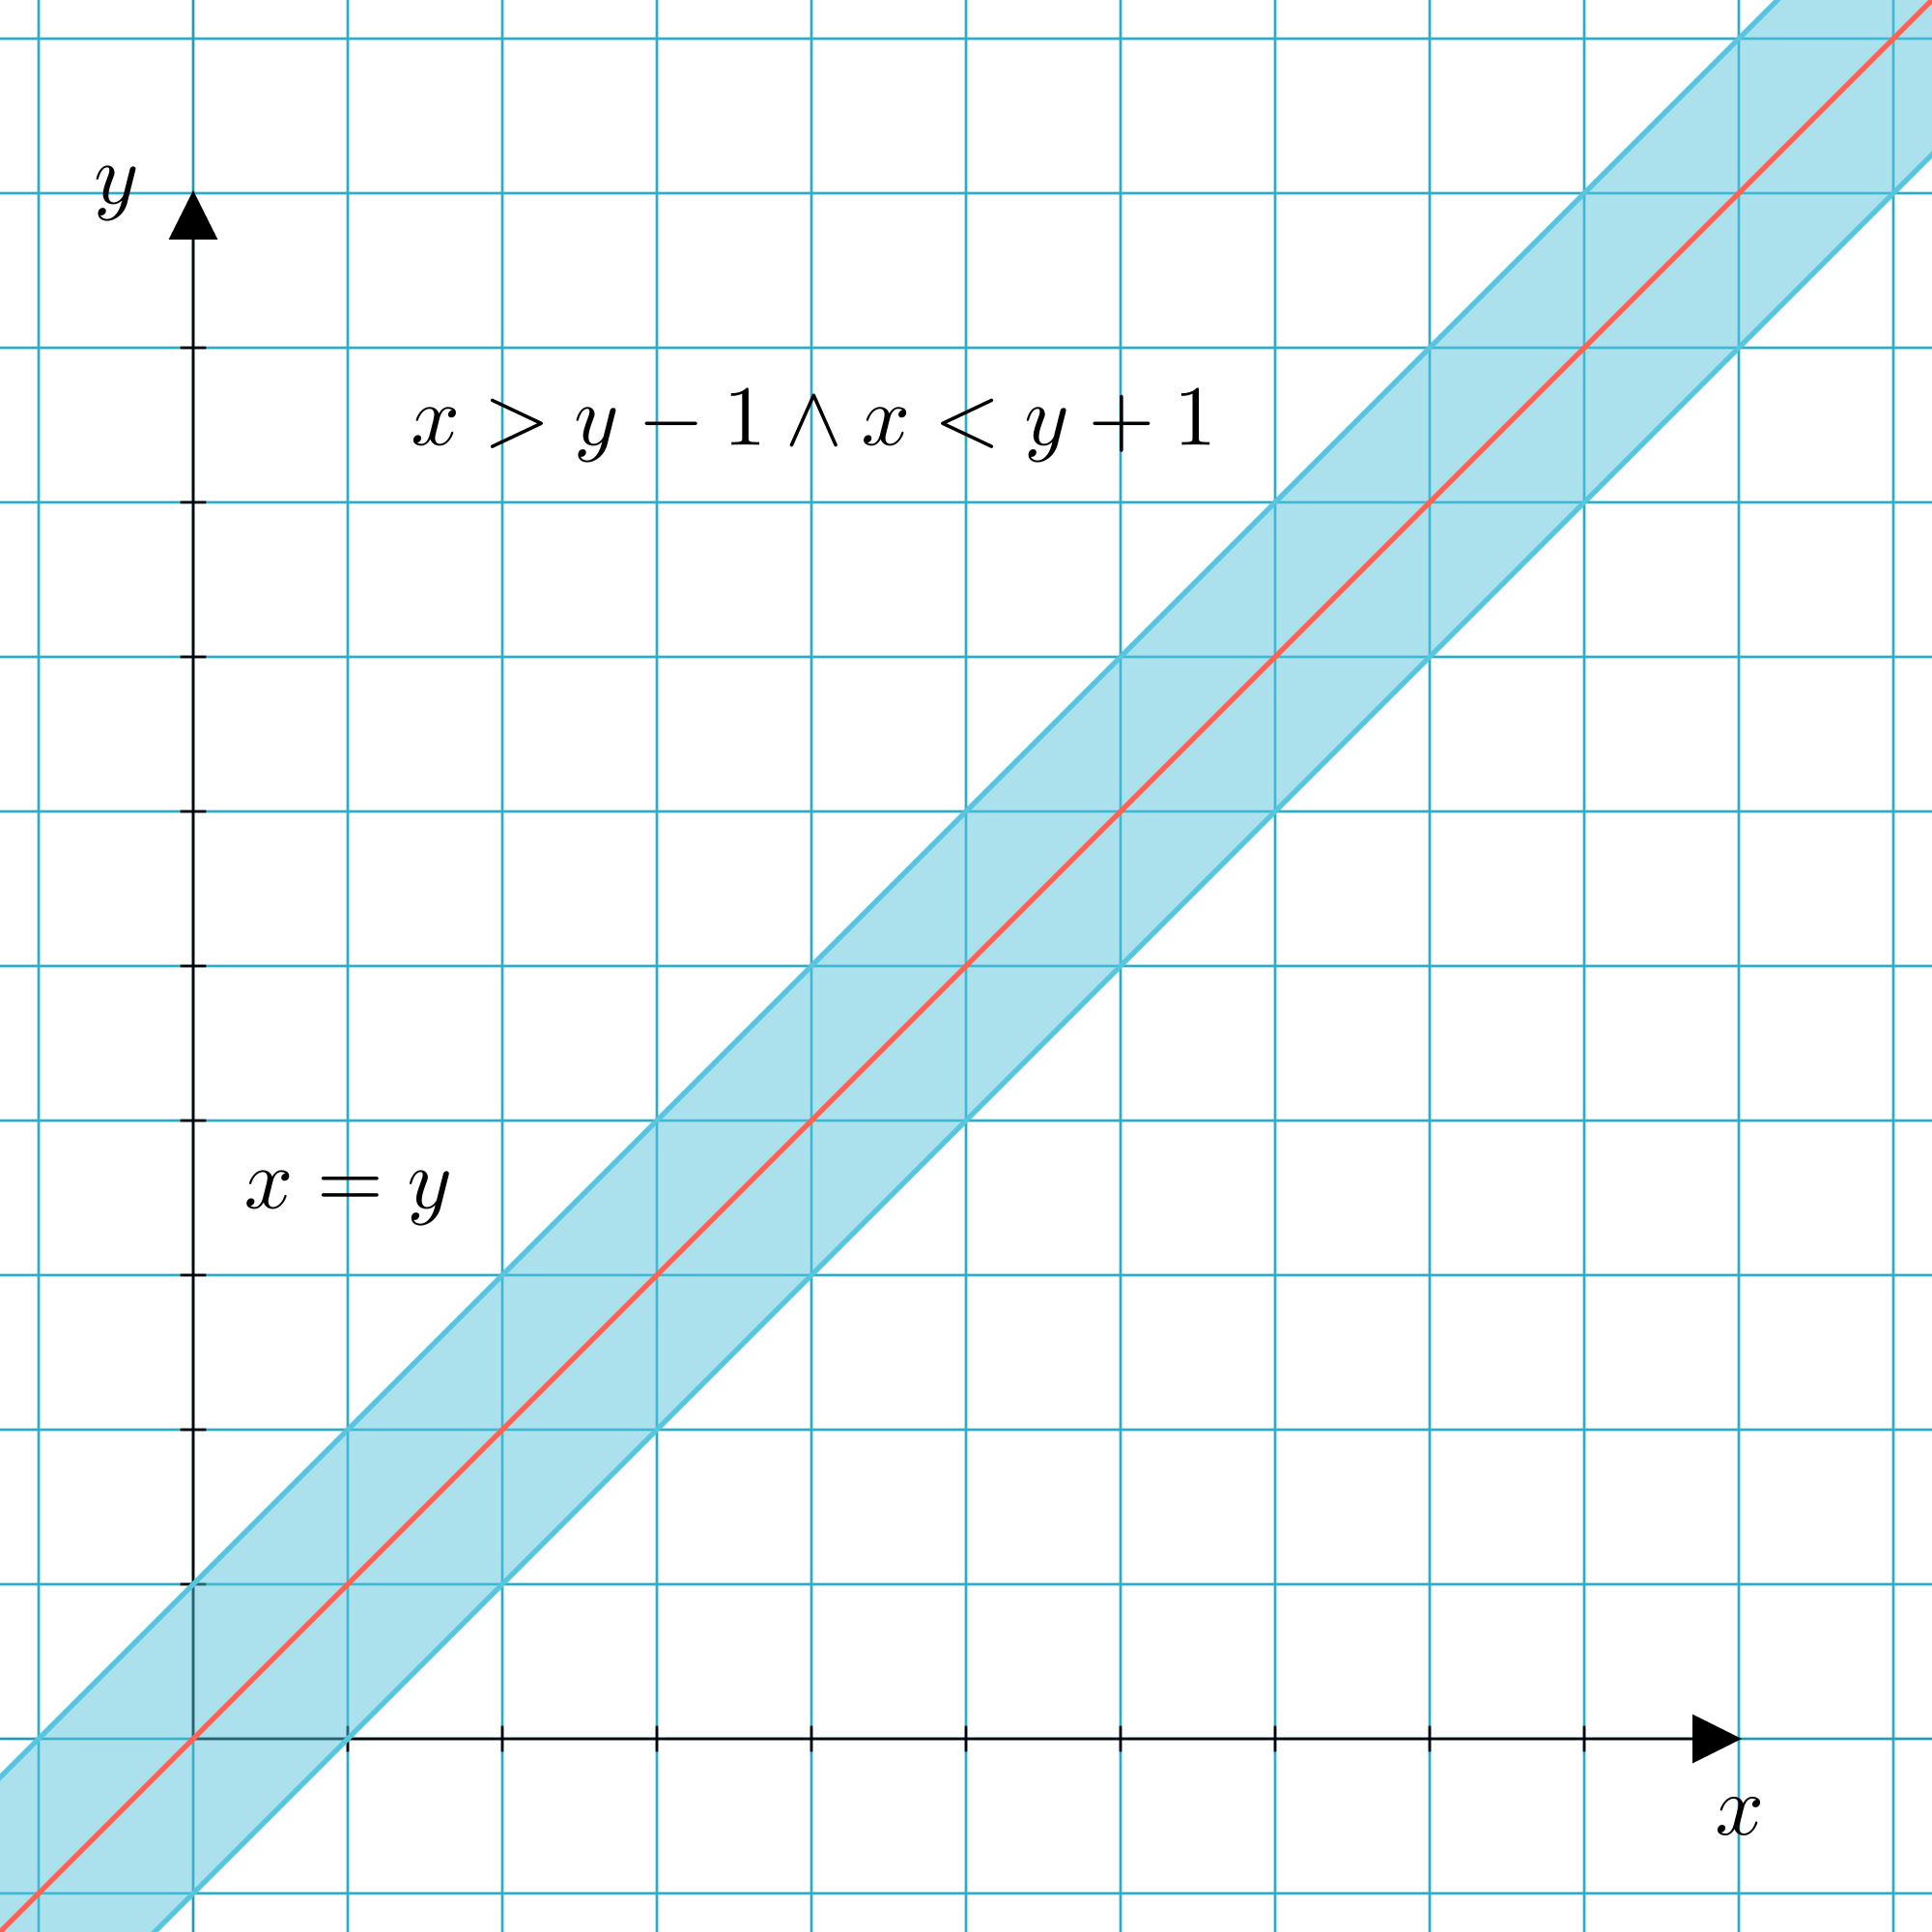
\includegraphics[width=0.4\linewidth]{../context-space.png}
	\caption{Figure showing a value space, where inclusion can not be shown}
	\label{fig:flux-context-space}
\end{figure}

The subtyping rules are quite similar. To the degree applicable, \textsc{S-Exists} is analogous to \textsc{$\preceq$-Ty}.

Looking at the choice of target language, we can see another difference: Flux chose $\lambda_{\text{Rust}}$ by Jung et al. \cite{jung_rustbelt_2018} as a basis for the formalization, which expresses the semantics in a continuation passing style over a language based on Rustc's MIR, which provides a more direct correspondence to the actual Rust.
On the other hand Corten based the formalization on a language based on Rustc's HIR and semantics expressed in a small-spec semantic. 

The corresponding implementations also use the MIR and HIR respectively. The advantages and disadvantages are discussed in \cref{ch:implementation}. Flux takes advantage of the MIR to cover a greater variety of control-flow scenarios.
Lehmann et al. also found that "the refinement annotations [..] do not appear in Rust's MIR" \cite[p. 17]{lehmann_flux_2022}, which poses a challenge for the implementation.

Lastly Lehmann et al. evaluate Flux against Prusti proving properties like "the absence of index-overflow error in a suite of vector-manipulating programs." \cite[p. 2]{lehmann_flux_2022}
Lehmann et al. found that the liquid type inference system is powerful enough to infer necessary invariants for this use case, partly because "loop invariants express either simple inequalities or tedious bookkeeping." \cite[p. 21]{lehmann_flux_2022}
In these cases Prusti still required invariants to be specified, which Lehmann et al. party attribute to the fact, for every unchanged mutable reference, the invariant needs to state that the reference was not modified. By using \code{mut}, but not \code{strg} references, Flux could avoid that problem.
Even though Corten does not share the the strong references mechanism with Flux, the argument still applies: Corten would also not require additional invariants for the unchanging mutable references.
Because Corten does not support vectors (yet), a direct comparison is not possible, but \cref{lst:evaluation-vec} approximates it.

